\begin{frame}
	\begin{figure}
		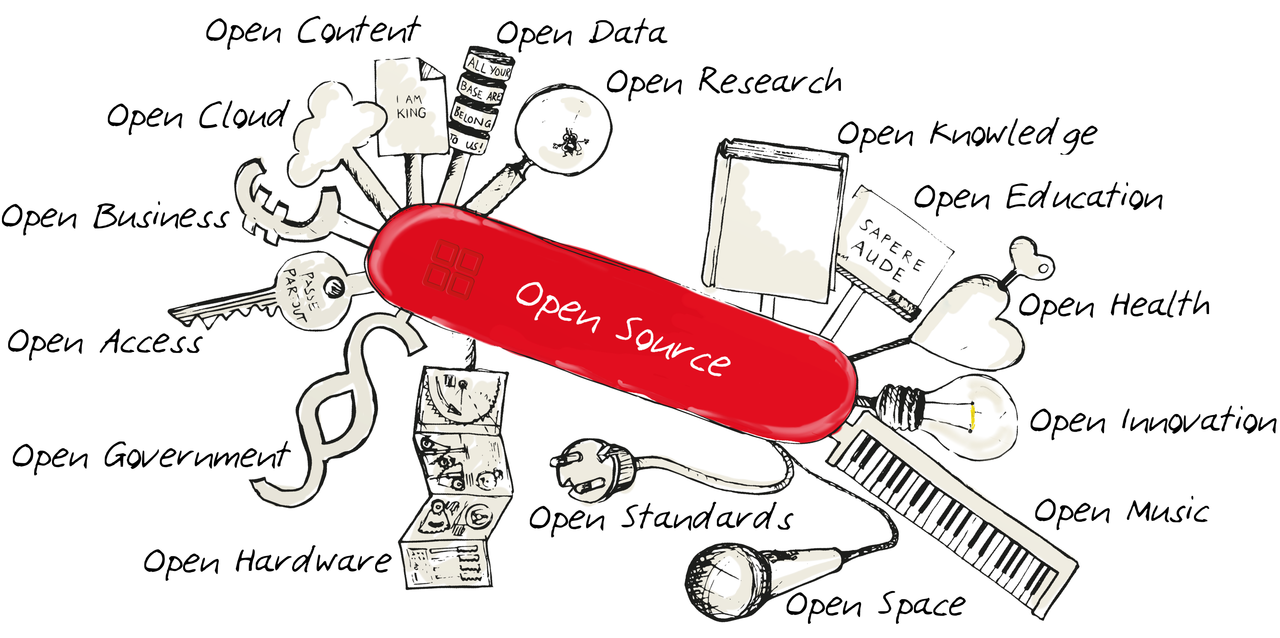
\includegraphics[scale=1]{resources/open_swiss_knife.png}
	\end{figure}
\end{frame}

\begin{frame}
\centering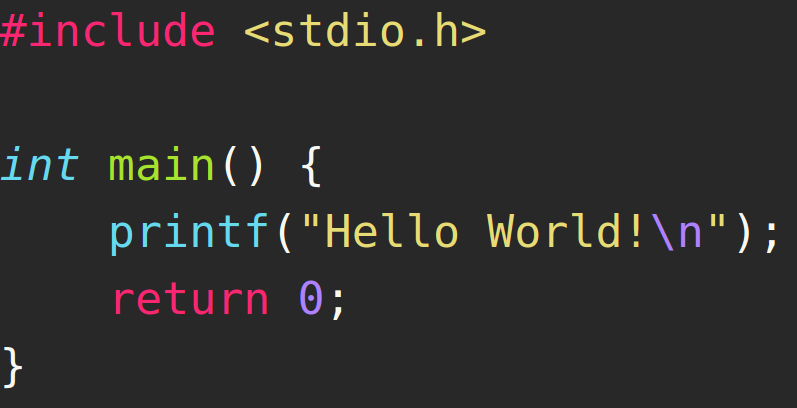
\includegraphics[scale=0.5]{resources/hello_world_code.png}
\end{frame}

\begin{frame}
\centering
\includegraphics[scale=0.3]{resources/hello_world_bin.png}
\end{frame}

\begin{frame}
	\frametitle{Warum ist Open-Source cool?}
	\begin{figure}
		
\includegraphics[scale=0.4]{resources/att.jpg}
	\end{figure}
	\begin{itemize}
		\item Fehlerbehebung durch Community
		\item Angriffspunkte werden frühzeitig erkannt
		\item Kontrolle bzgl. unerwünschter Nebenfunktionen
	\end{itemize}
\end{frame}

\begin{frame}
	\begin{figure}
		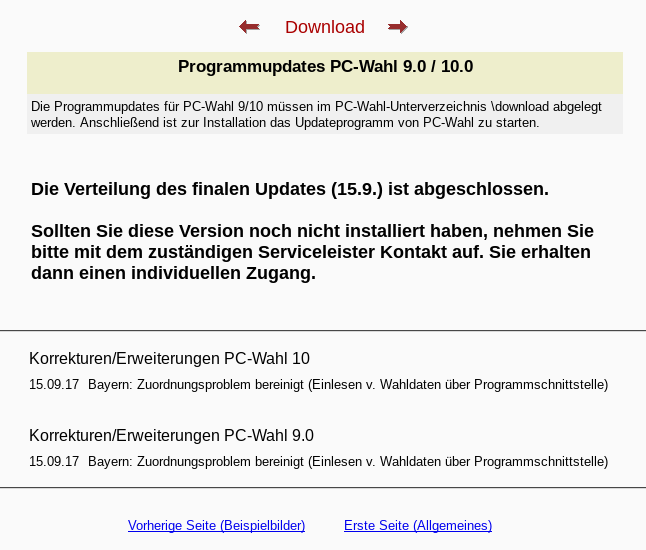
\includegraphics[scale=0.4]{resources/pcwahl10.png}
	\end{figure}
\end{frame}

\begin{frame}
	\begin{figure}
		
\includegraphics[scale=0.45]{resources/pmpc.png}
	\end{figure}
\end{frame}